\documentclass{article}
\author{Szymon Stefański}
\title{Ćwiczenie}
\usepackage{graphicx}
\usepackage{amsmath}
\usepackage{fullpage}
\usepackage{hyperref}
\begin{document}
\maketitle
\begin{equation}
    e^{i\pi}=-1 \label{Euler}
\end{equation}
\eqref{Euler} na stronie \pageref{Euler}
\footnote{
\url{https://www.agh.edu.pl/o-agh/historia-i-tradycja}
\href{https://www.agh.edu.pl/o-agh/historia-i-tradycja}{test}}
\begin{figure}
    \centering
    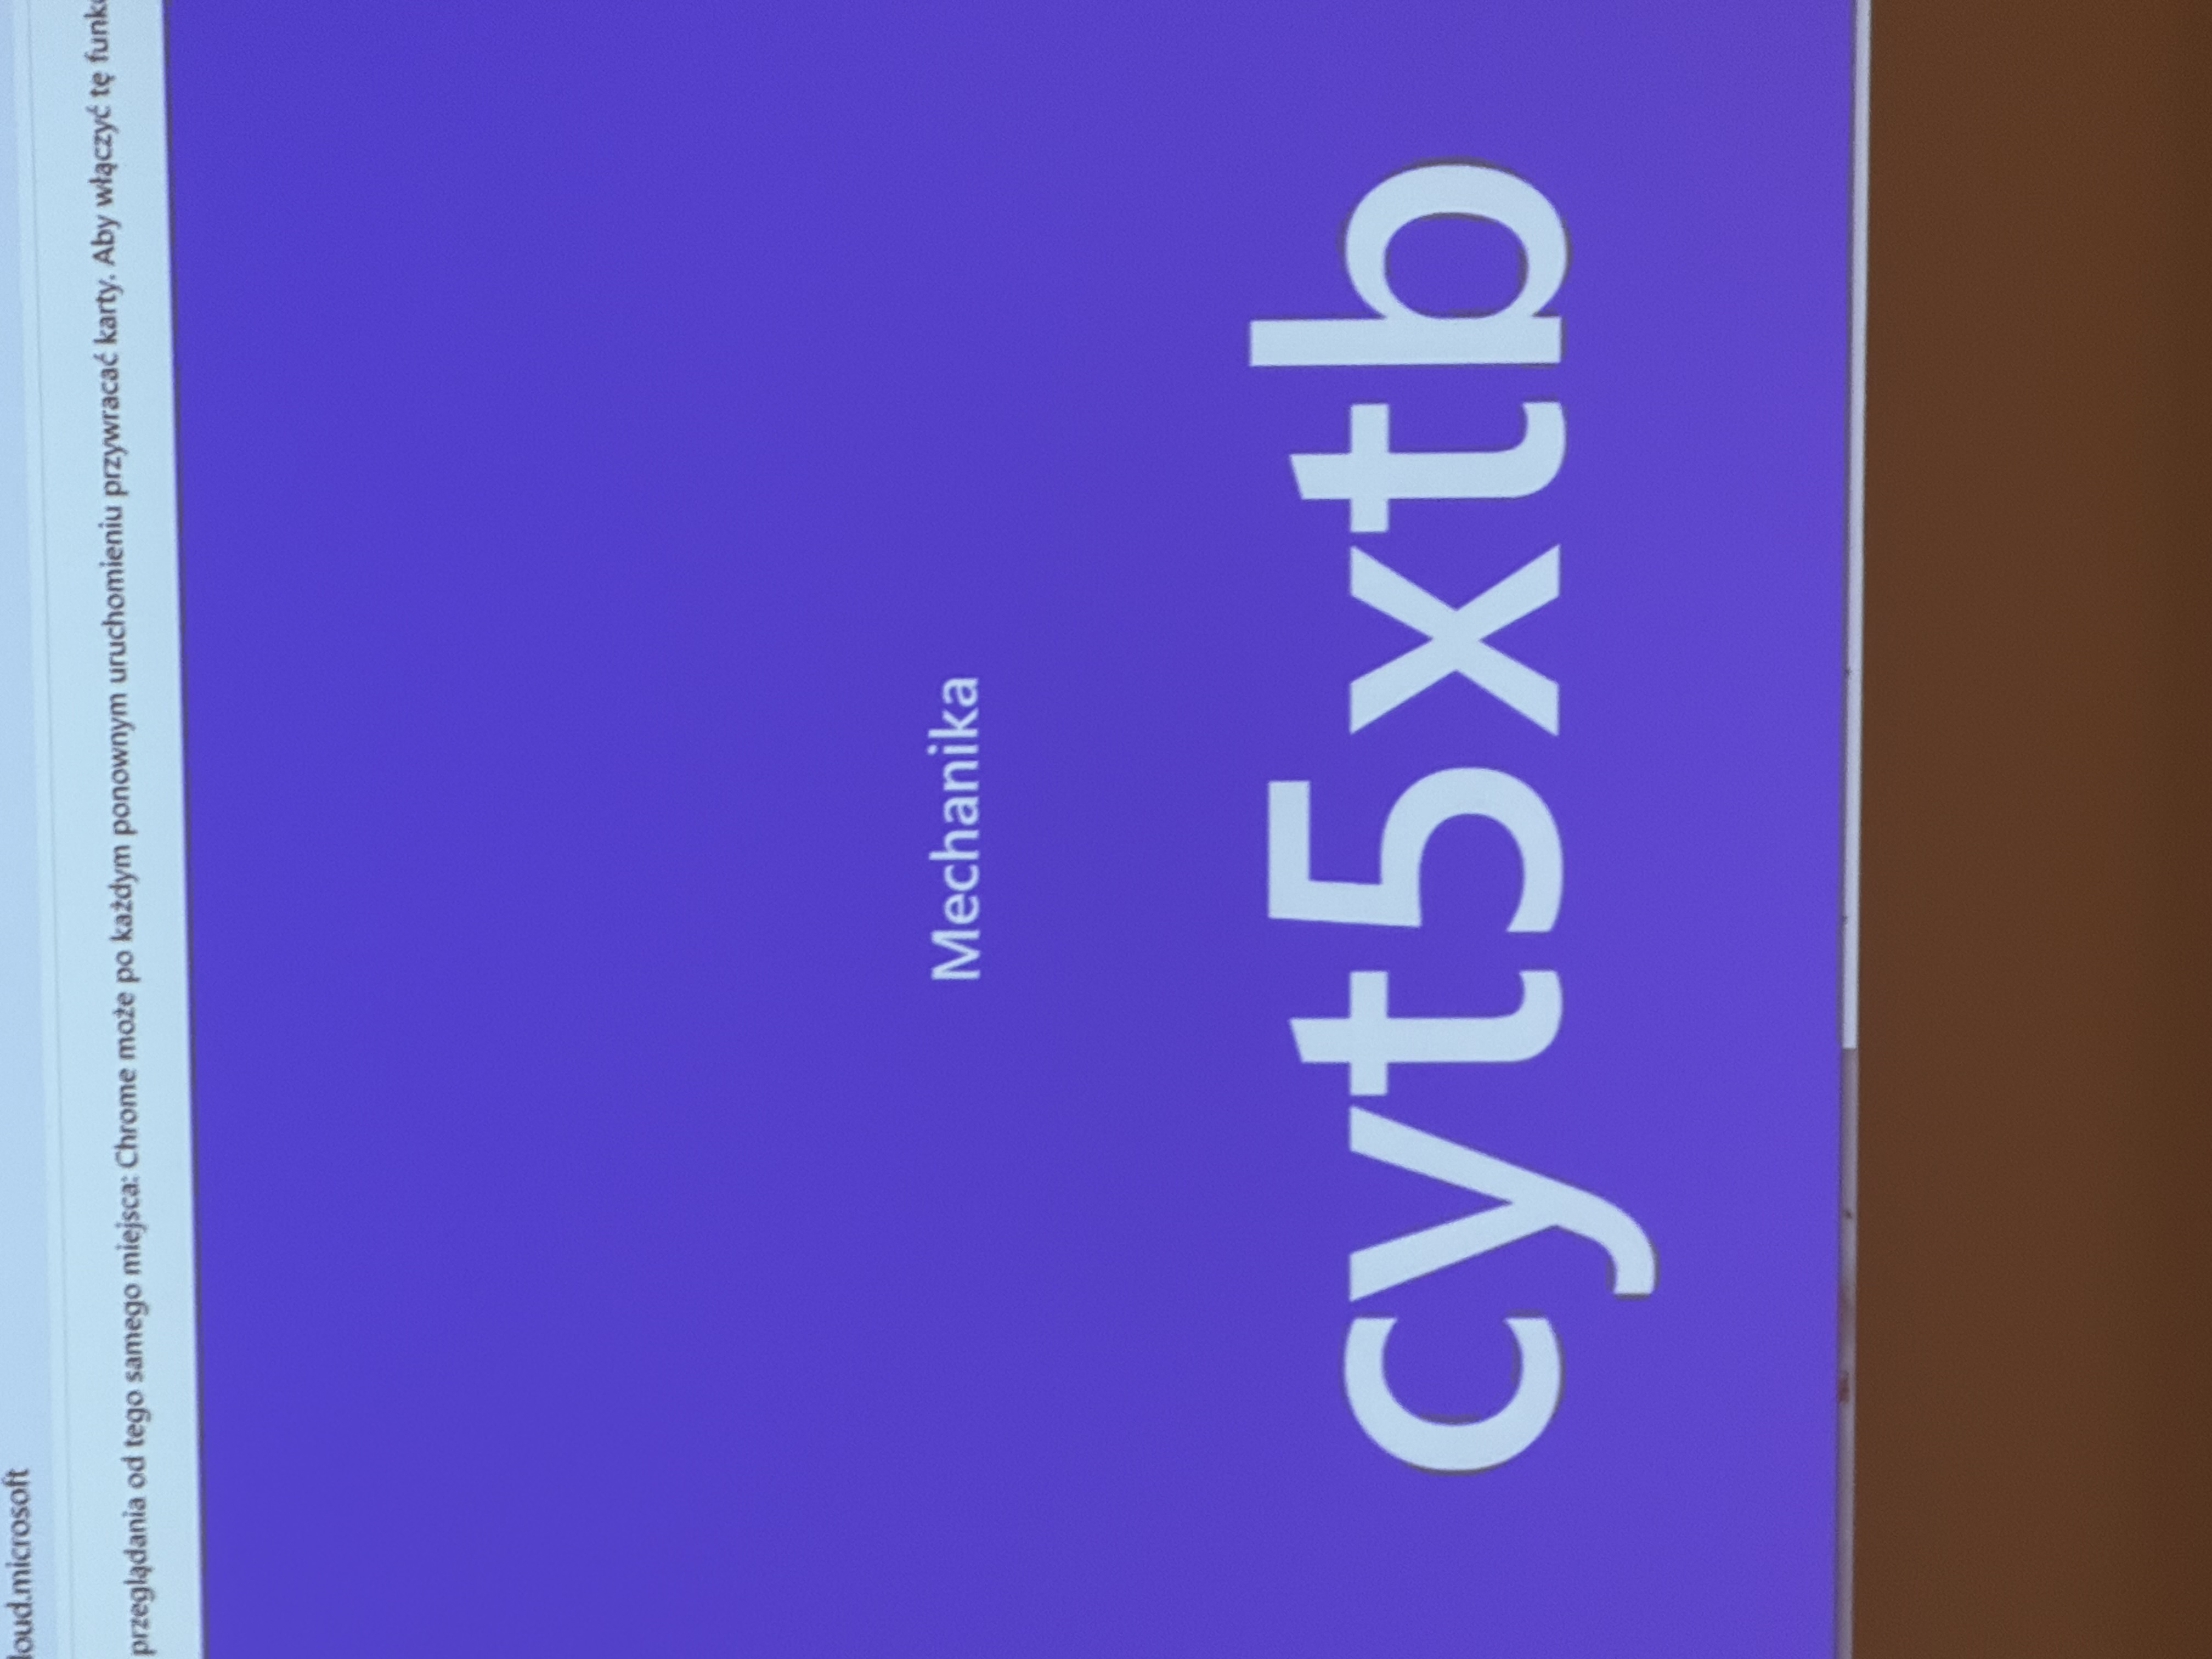
\includegraphics[width=0.5\linewidth]{IMG_2728.jpeg}
    \caption{Zdjecie}
    \label{fig:placeholder}
\end{figure}
\end{document}